\documentclass[12pt]{article}
\usepackage[hmargin=1in, vmargin=1in]{geometry}
\usepackage{fancyhdr}
\pagestyle{fancy}
\usepackage{lastpage}
\usepackage{graphicx}
\DeclareGraphicsExtensions{.jpg}
\usepackage{url}

\def\author{Jacques Uber}
\def\title{FredMeyer Camping Headlamp}
\def\date{\today}

\fancyhf{} % clear all header and footer fields
\fancyhead[LO]{\author}
\fancyhead[CO]{\title}
\fancyhead[RO]{\date}
% The weird spacing here is to get the spacing of \thepage to be right.
\fancyfoot[C]{\thepage\
                    / 5}

\setcounter{secnumdepth}{0}
\setlength{\parindent}{0pt}
\setlength{\parskip}{4mm}
\linespread{1.4}

\begin{document}
The FredMeyer headlamp is a pocket sized light source designed for wearing around one's head during
situations when visibility could be aided by a supplementary light source. The headlamp is made up
of two parts: the lamp, and the strap. The lamp has three settings allowing for light of different
color to be emitted from the bulbs.

\begin{figure}[h!]
\centering
\caption{Head lamp from the front.}
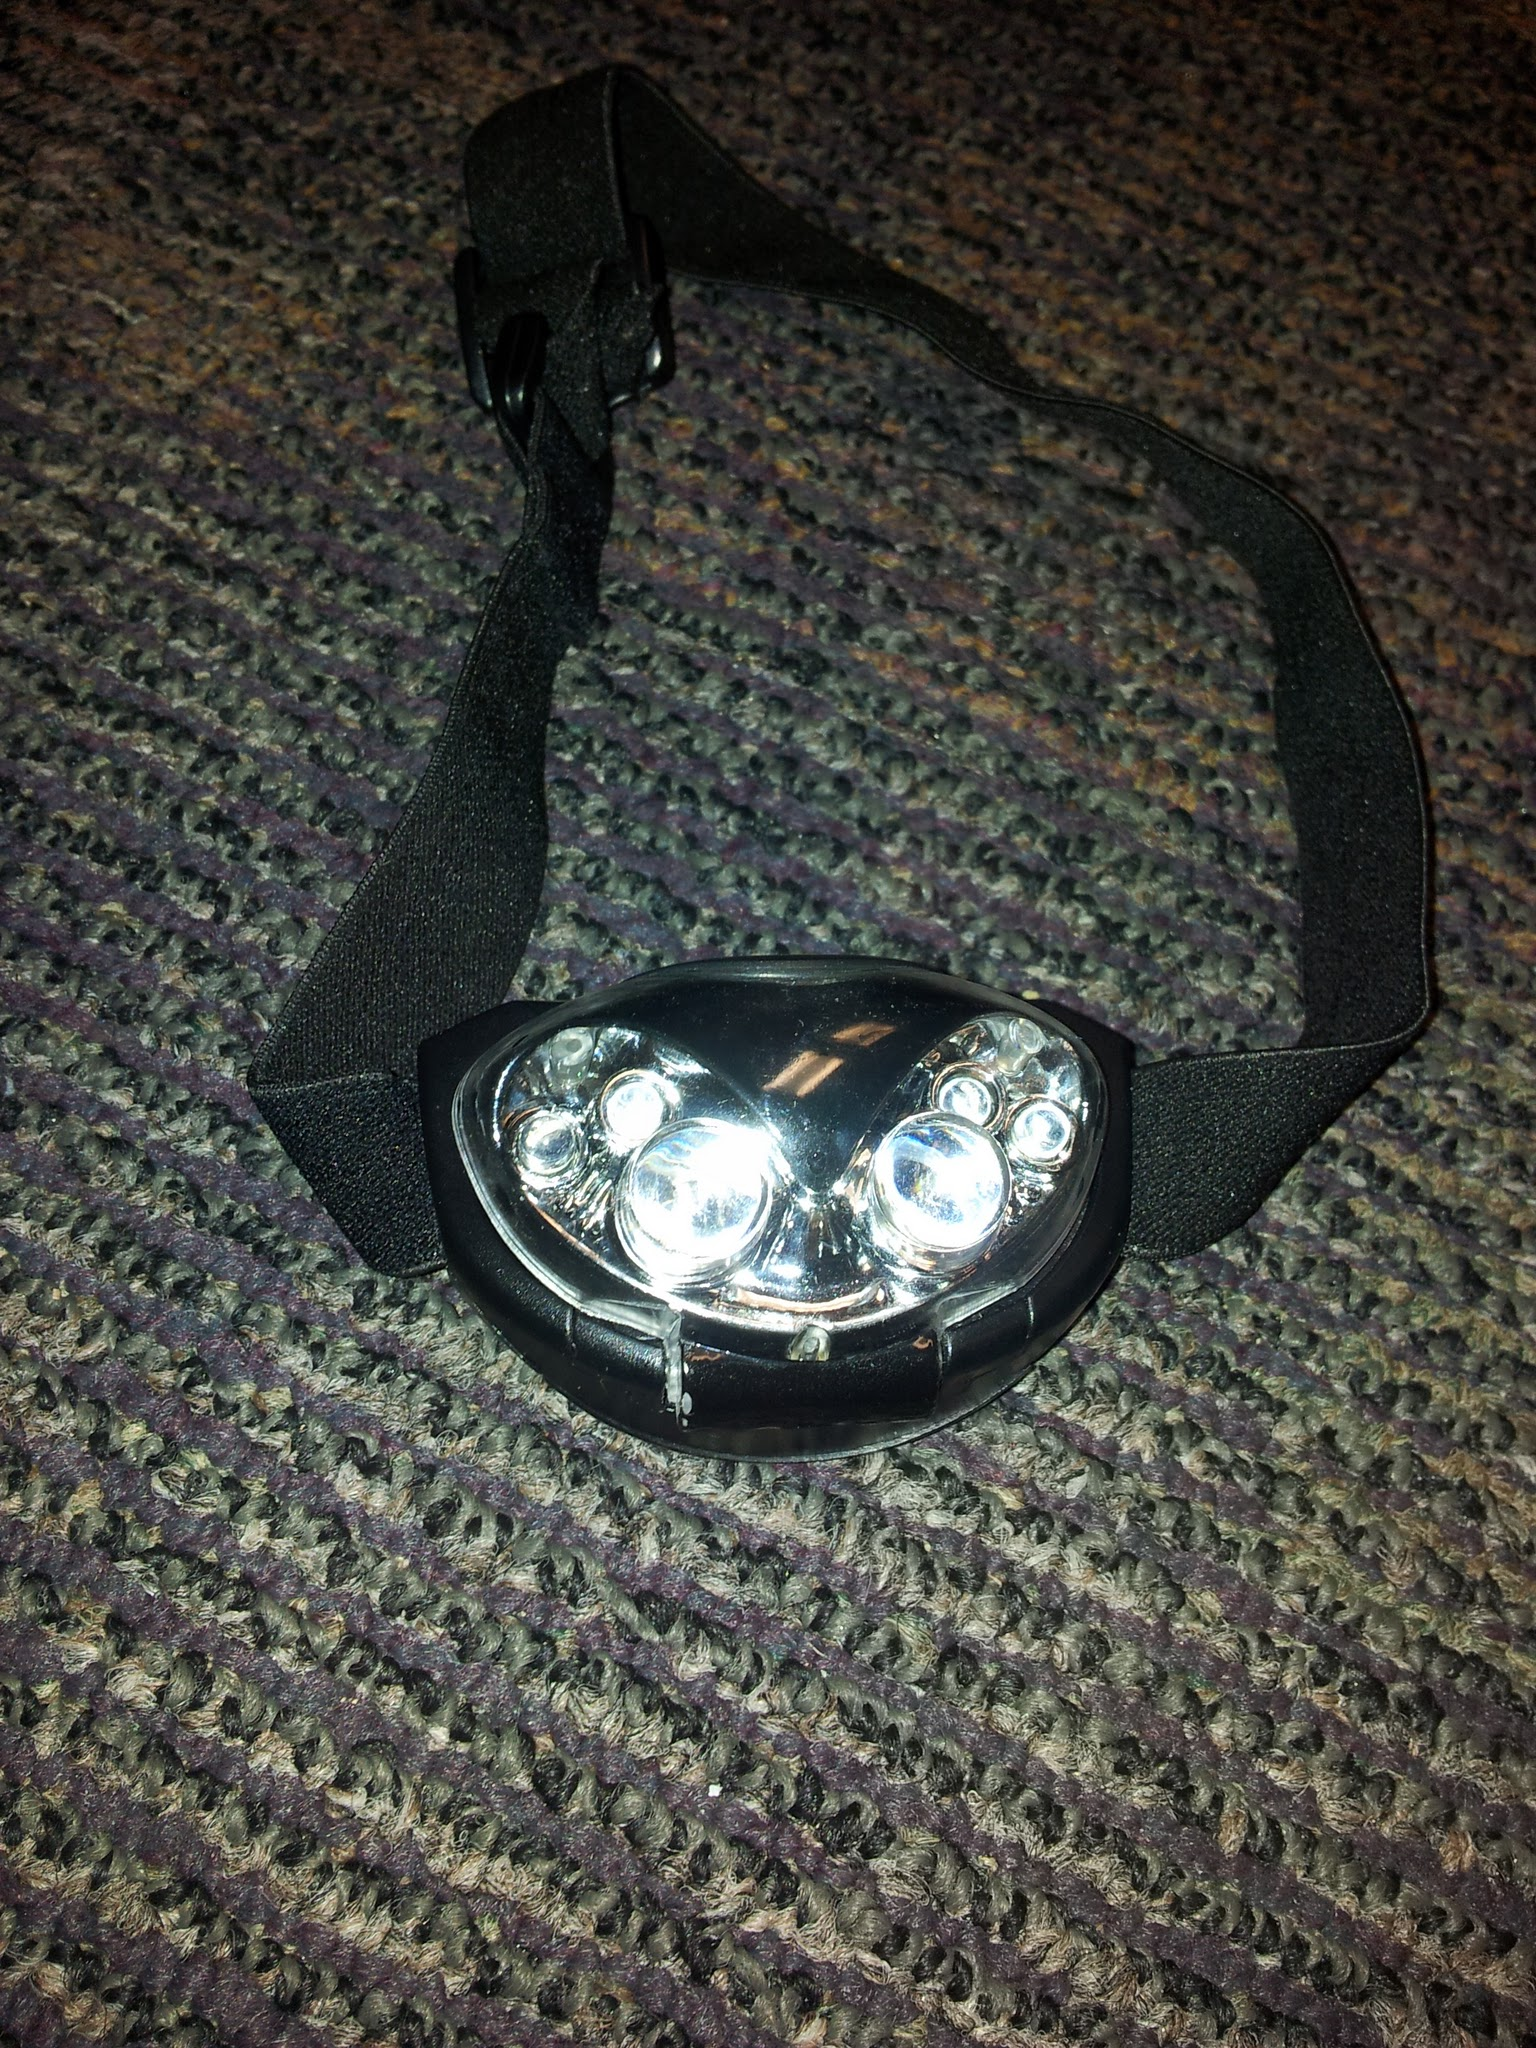
\includegraphics[width=3in]{headlamp}
\end{figure}

\begin{figure}[h!]
\centering
\caption{Head lamp from the side.}
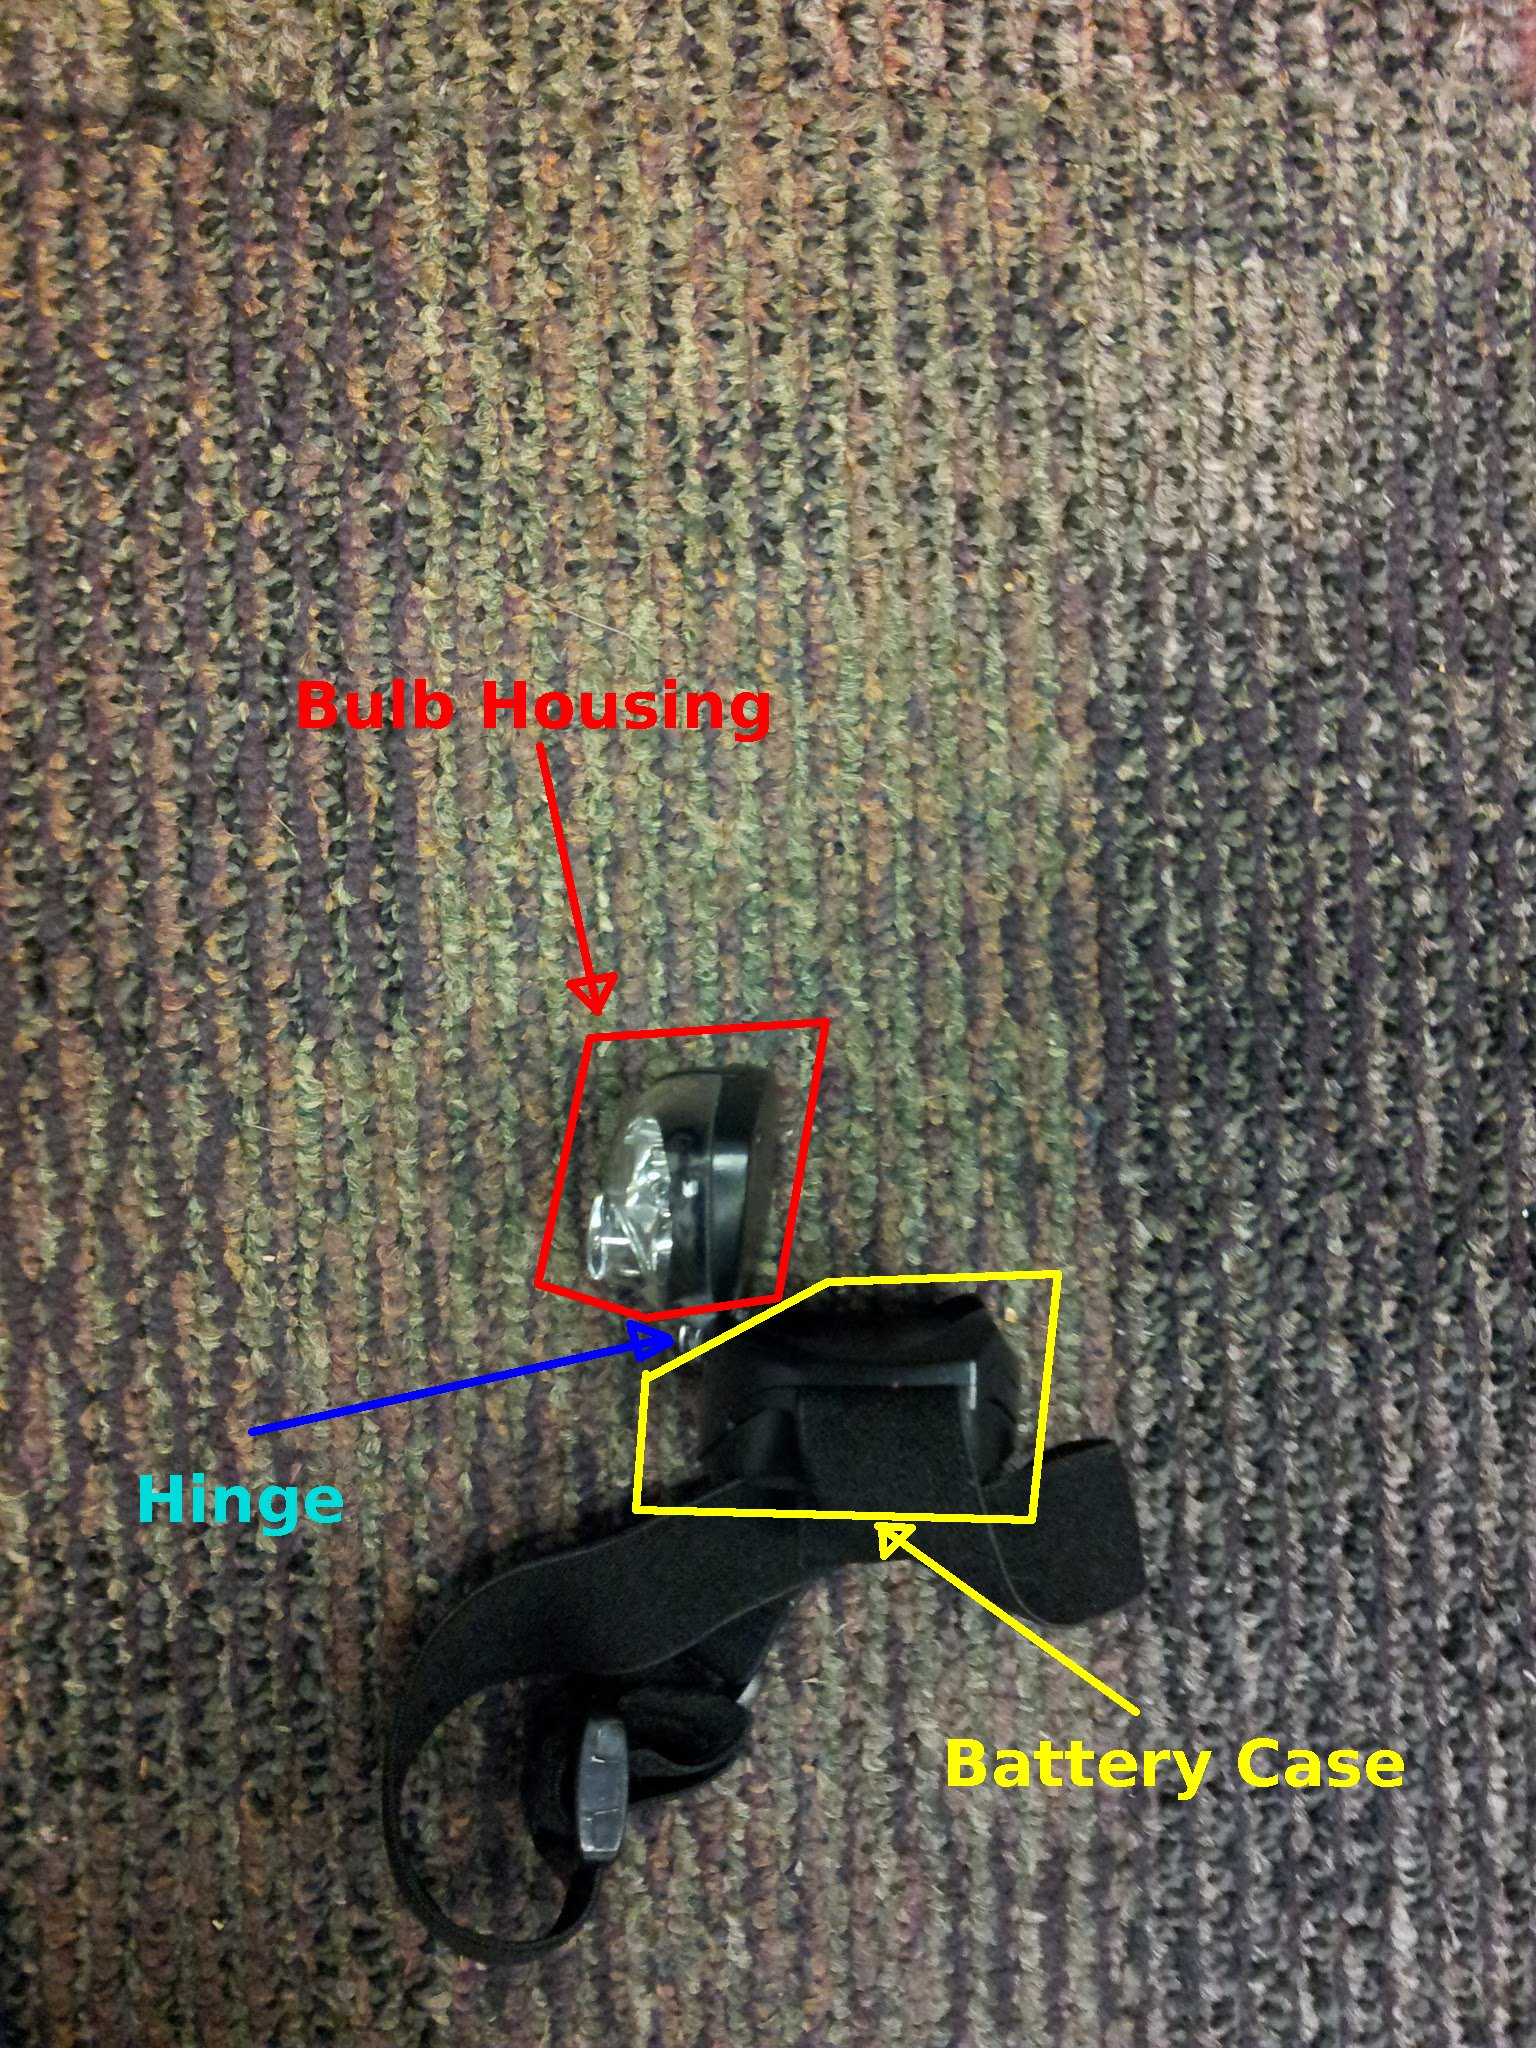
\includegraphics[width=3in]{headlamp_side}
\end{figure}

\begin{figure}[h!]
\centering
\caption{Head lamp from the top.}
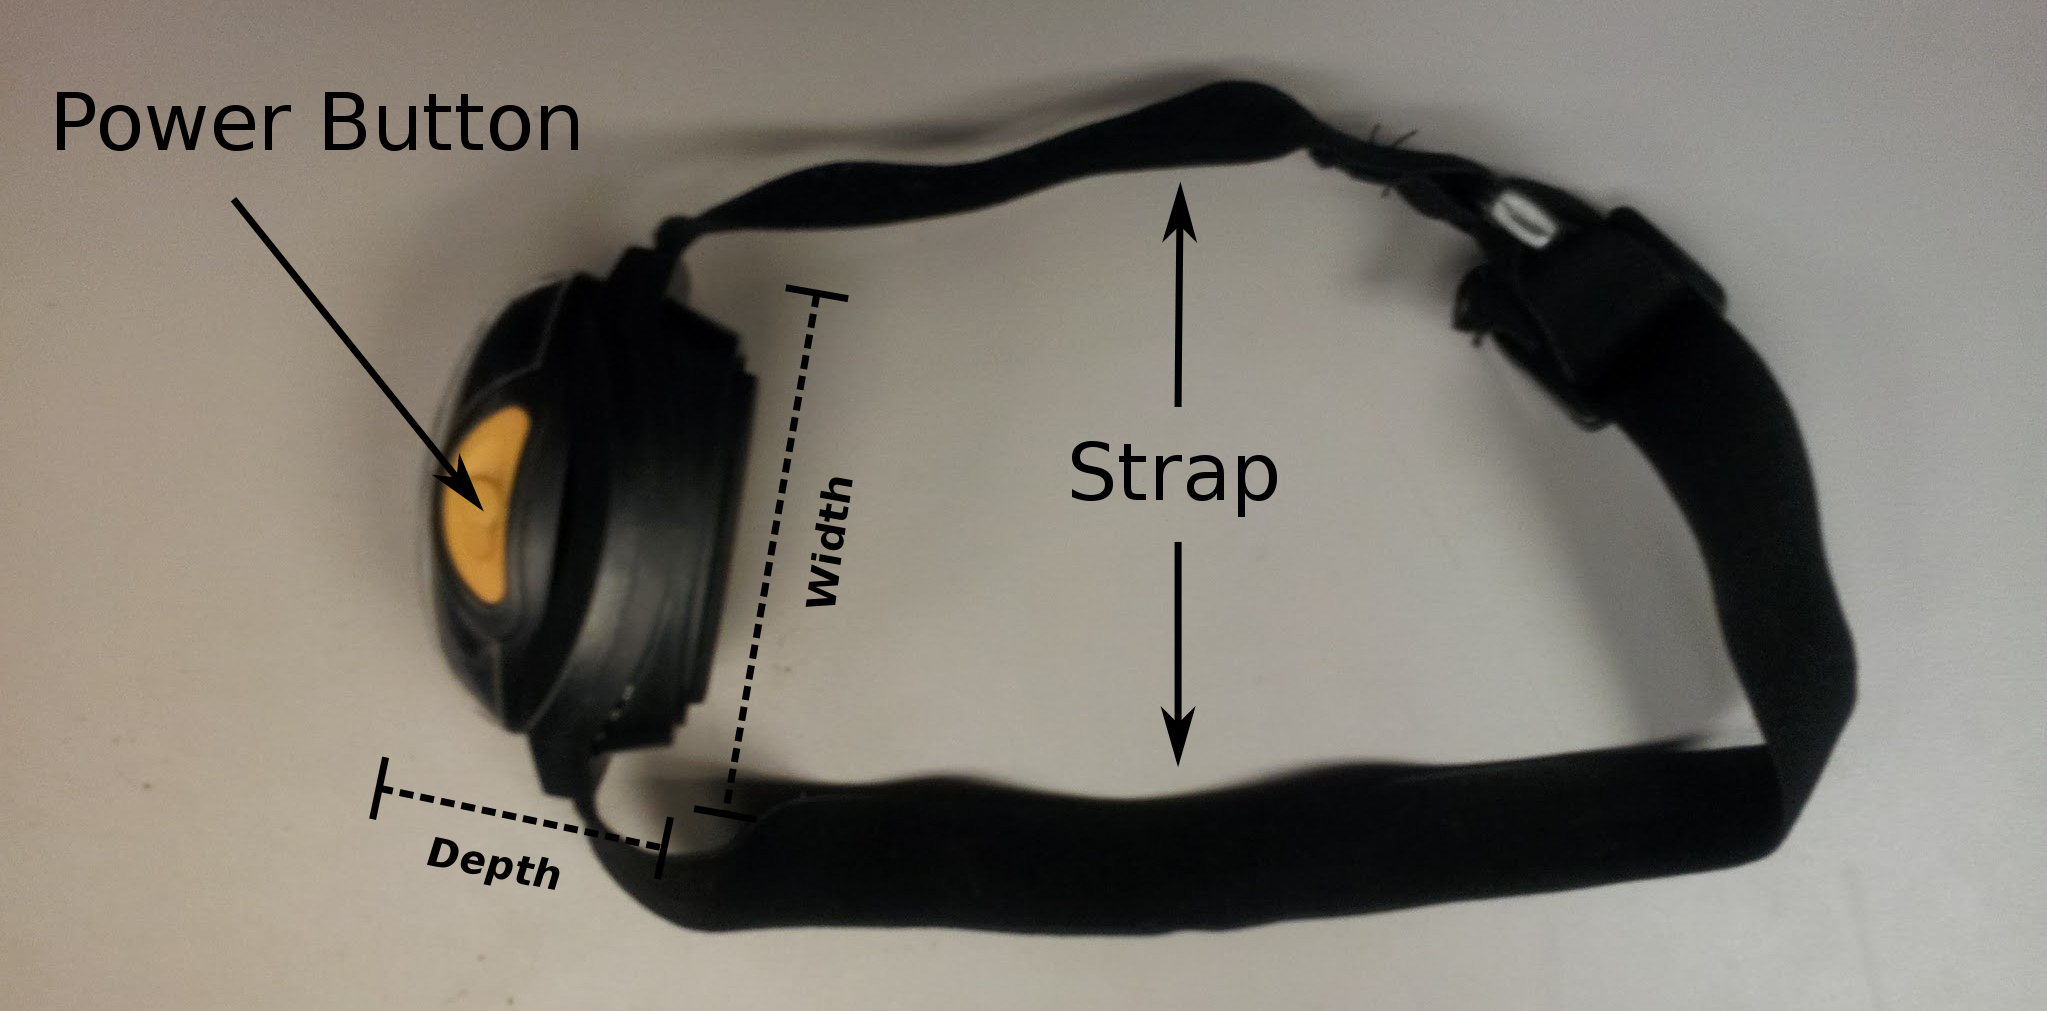
\includegraphics[width=3in]{headlamp_top}
\end{figure}

\section{The Lamp}
The lamp preforms the primary function of the headlamp. It is roughly 1/4 pounds when loaded with
it's 3 AAA battery power source. The lamp itself is split into two modules: the bulb housing and the
battery case. The two modules are joined by a hinge which allows the LEDs (Light Emitting
Diodes) to be aimed variably. (figure 2)

\subsection{Bulb housing}
The bulb housing module holds the LEDs, LED casing, and power switch.

\subsubsection{LEDs}
The lamp has 6 main LEDs, 4 of the LEDs are white and the remaining 2 are red (figure 1). Of the 4
white LED's 2 of them have a radius of 0.5cm and are located symmetrically opposite of each other
located 1cm away from the front center line of the lamp.  The remaining 4 LEDs have a radius of
0.25cm and are aligned symmetrically opposite to each other and are lined up starting 2cm away from
the front center line of the lamp. With regard to the 4 0.5cm LEDs, the two furthest from the center
line are white, the inner pair are red.

\subsubsection{LED Casing}
To protect the LEDs, a clear form fitting case covers the front of the lamp.  The case also acts to
focus and intensify the light from the LEDs. The case consists of hard plastic and is roughly
3mm thick.

\subsubsection{Power Toggle}
Turning on the lamp is done with a plastic yellow power toggle located on the top of the lamp
directly above the casing and LEDs (figure 3). The toggle is pressure sensitive.

\subsection{Battery Case}
The majority of the headlamp is used to house the power supply. The supply case is rectangular with
rounded edges (figure 2). It is 5cm across, 3cm wide, and 1.5cm deep. When in use the back of the case is
placed on to the users forehead. To make this more comfortable there is a soft black padding on the
back 5cm by 3cm panel.

\section{The Strap}
The strap serves the function of holding the headlamp to the users head. The variable length strap
is at maximum 2 feet long, and at minimum 1/2 foot long (figure 3). It is made of an elastic material that
is black. The elasticity of the strap allows a strip of contracted material to be stretched into a
strip 2 times it's original length.

\section{Bulb settings}
The LEDs can be configured via the power toggle to emit three forms of light: Normal-White,
Bright-White, and Flashing-Red. These settings are achieved by powering some LEDs while not
powering others.

\subsection{Normal-White}
From the off state, toggling power once will place the headlamp into the Normal-White state.  This
setting drives power to the two main, 0.5cm radius, LEDs.

\subsection{Bright-White}
From the off state, toggling power twice will place the headlamp into the Bright-White state.  This
setting drives power to both the two main, 0.5cm radius, LEDs and the two outer white, 0.25cm radius, LEDs.

The headlamp emits the most light while in this state.

\subsection{Flashing-Red}
From the off state, toggling power three times will place the headlamp into the Flashing-Red state.
This setting drives power to the two inner, 0.5cm radius, red LEDs. While in this state the
LEDs will flash on and off at a frequency of 3 times per second. Each flash has a duration of
0.25 seconds.


\end{document}
